\chapter{Methoden} 
\label{chapter:meth}

In diesem Kapitel werden für die in Kapitel \ref{chapter:mod} vorgestellten Modelle Möglichkeiten beschrieben, diese zu simulieren. 
Zunächst werden zwei Herangehensweisen erläutert, das 2-Zustände und das 3-Zustände Modell als Simulation vieler Einzelteilchen umzusetzen.

Im zweiten Abschnitt des Kapitels wird beschieben, wie der PAA umgesetzt werden kann. Dabei liegt der Fokus auf einer eingeschränkten Variante des PAA, bei dem einige nicht benötigte Funktionalitäten, wie beispielsweise je Zustand verschiedene Operationen oder mehrere mögliche Emissionen, nicht berücksichtigt werden.

Die Ankunftszeiten der simulierten Teilchen bzw. die Verteilung der Wartezeiten auf das Erreichen der Säulenlänge, können dann als Peak aufgefasst und dargestellt werden. Wie aus diesen Daten außerdem werden die resultierenden Peakdaten berechnet werden können, steht im letzten Abschnitt beschrieben.

\section{Simulation}
Offensichtlich ist es möglich, tatsächlich jeden einzelnen Zeitschritt für alle Teilchen zu betrachten. Jedes Teilchen durchläuft also den Automaten aus Abbildung \ref{tikz:2p_Mod} und es wird in jedem Schritt entschieden, ob es sich fortbewegt. Diese schrittweise Art der Simulation wird im Folgenden als ``Step-by-Step'' bezeichnet.

Wenn Zustandswechsel jedoch nicht sehr häufig vorkommen, kann es viel Zeit einsparen, nur zu relevanten Zeitpunkten, also für jeden Zustandswechsel, zu simulieren und dabei den Zeitpunkt des nächsten Wechsels zu notieren. Diese Zeitpunkte werden als Ereignisse verwaltet, daher wird diese Art der Simulation im Folgenden auch ``By-Event'' genannt.

%Zunächst betrachten wir das in \ref{chapter:mod:2p} vorgestellte Modell mit nur zwei Zuständen und zwei Parametern, anschließend auch die in \ref{chapter:mod:3s} beschriebene Erweiterung auf 3 Zustände und damit bis zu 6 Parameter. Eine Unterscheidung zwischen Modell 3a und 3b findet hier nicht statt, sondern es werden beide zu einem allgemeinen Modell zusammen gefasst. Für die jeweilige Umsetzung müssen dann einfach die zwei nicht benötigten Übergangswahrscheinlichkeiten auf $0$ gesetzt werden.

%Nach erfolgter Simulation können aus den Ankunftszeiten der Teilchen die Peakdaten der resultierenden Peaks berechnet werden.

%Für das 2-Zustände Modell wurden zwei verschiedene Möglichkeiten der Simulation entworfen. Die erste, ``Step-by-Step'', simuliert schrittweise alle Zeitpunkte eines Säulendurchlaufs. Die zweite, ``By-Event'' verwaltet eine Liste relevanter Zeitpunkte, an denen Ereignisse - im konkreten Fall: Zustandswechsel - statt finden.
\subsection{Step-by-Step}

\begin{algorithm}
\caption{Ablauf der Step-by-Step Simulation}
\label{algo_by_Step}
\begin{algorithmic}
\REQUIRE Zustandsliste $z= [z_1 , \ldots, z_n]$, Ortsliste $o=[o_1, \ldots , o_n]$, Zeit $t=0$, Maximalzeit $t_{max}$, Transitionen $T$
\ENSURE Ankuftszeiten $r$ oder FAIL
\WHILE{$t < t_{max}$ \AND $len(z) > 0$}
\FORALL {Teilchen $p$}
\STATE Simuliere $p(T)$
\IF {$o_p >l$}
\STATE $r \leftarrow t$
\STATE Lösche $z_p$ und $o_p$
\ENDIF
\ENDFOR
\STATE $t +=1$
\ENDWHILE
\IF {$len(z) > 0$}
\RETURN FAIL
\ELSE
\RETURN $r$
\ENDIF
\end{algorithmic}
\end{algorithm}

%\todo{Hinweis auf Parallelisierbarkeit und andere Zeitverbesserungen hier oder in Implementierung}

Der Ablauf einer schrittweisen Simulation ist in Algorithmus \ref{algo_by_Step} gegeben und unterscheidet sich zunächst nicht für das 2-Zustände und 3-Zustände Modell.

Simuliert werden $n$ Teilchen. Für jedes Teilchen $p$ muss jeweils der aktuelle Zustand $z_p$ und Ort $o_p$ festgehalten werden, außerdem muss in jedem Schritt der aktuelle Zeitpunkt $t$ vermerkt werden. Die Zustände $z_p$ und Orte der Teilchen $o_p$ %\in \{0, \ldots, \ell\}$ 
werden jeweils in einem Array festgehalten. Die Identifikation der Teilchen geschieht dabei über ihre Postition, die in beiden Arrays identisch ist.
%\todo{Array oder Vektor, bzw ohne Parallelisierbarkeit, da ja eigentlich nicht nötig?}
%Für jedes Teilchen wird in einem zweiten Array an gleicher Position sein aktueller Ort gespeichert. 

Simuliert wird, bis alle Teilchen das Säulenende erreicht haben, also die Vektoren eine Länge von $0$ haben. 
Als alternative Abbruchbedingung kann eine maximale Anzahl von Simulationsschritten gewählt werden, nach deren Ablauf die Simulation beendet ist, wenn nur Peaks von Interesse sind, die vor diesem Zeitpunkt im Chromatogramm erscheinen.

Es wird nun jeweils ein Zeitschritt für alle Teilchen simuliert. Nach jedem solchen Simulationsschritt wird getestet, ob Teilchen bereits den Wert von $\ell$ erreicht und damit die ganze Säule durchlaufen haben. Die entsprechende Anzahl dafür benötigter Schritte entspricht der Ankunftszeit der Teilchen und wird festgehalten, sodass als Ergebnis am Ende der Simulation eine Liste von Ankunftszeiten aller Teilchen entsteht. Teilchen, die angekommen sind, werden aus beiden Vektoren gelöscht.

Wenn die Simulation für alle Teilchen zu Ende geführt wurde, ist die Rückgabe die Liste der Ankunftszeiten aller Teilchen. Ansonsten gilt die Simulation als gescheitert, die Parameter $p_{\text{s}}$ und $p_{\text{m}}$ sorgen offenbar nicht für einen vollständigen Peak innerhalb des simulierten Zeitraumes.

\subsubsection{Simulation des 2-Zustände Modells}

Da nur zwei Zustände existieren und für alle p gilt $z_p \in \{0,1\}$, bietet es sich an, als Zustandsvektor ein Array mit booleschen Werten zu verwenden. $0$ steht dabei für stationär und $1$ für mobil.

Die Berechnung eines Simulationsschrittes läuft wie folgt: Die Teilchen wechseln in jedem Schritt mit einer bestimmten Wahrscheinlichkeit den Zustand. Diese sei wie in Kapitel \ref{chapter:mod} erwähnt, $p_{\text{m}}$ für das Verweilen in der mobilen Phase, $p_{\text{s}}$ für das Verweilen in der stationären Phase und $1-p_{\text{m}}$ bzw. $1-p_{\text{s}}$ für die beiden Möglichkeiten des Phasenwechsels. Daher muss pro Schritt und Teilchen eine Zufallszahl gezogen werden, anhand derer sich entscheidet, wie es sich verhält. Außerdem muss in jedem Schritt der Ort für jedes mobile Teilchen um eins erhöht werden.

Zum Ablauf der Simulation wurde entschieden, dass zunächst die Entscheidung über die Phase gefällt wird und sich die Teilchen anschließend gemäß ihres neuen Zustandes bewegen. Alle Teilchen starten ganz zu Beginn in der mobilen Phase, da sie nur so in das System eintreten können. Außerdem beginnen sie an Ort $1$, da sie bereits als in der Säule befindlich angenommen werden. Das heißt, die Eingaben für Algorithmus \ref{algo_by_Step} sind $z= [z_1 = 1, \ldots, z_n=1]$ für die Zustände und $o= [o_1 = 1, \ldots, o_n=1]$ für die Orte.

\begin{figure}
\begin{tikzpicture}[->,>=stealth',shorten >=1pt,auto,node distance=4cm,
  thick,main node/.style={circle,fill=white!20,draw,font=\sffamily\large\fseries}]
\tikzstyle{feld}=[draw,minimum width=1.5cm,minimum height=0.7cm,font=\sffamily\footnotesize]

\begin{scope}[start chain =1 going right, node distance =0.0mm]
	\node [on chain =1, feld, draw=none,minimum width=2.5cm] {Phasen $z$};
	\node [on chain=1, feld, fill=blue!30!white] (p1) {0};
	\node [on chain=1, feld] (p3) {0};
	\node [on chain=1, feld, fill=green!30!white] (p4) {1};
	\node [on chain=1, feld] (p5) {1};
	\node [on chain=1, feld,fill=magenta!70!blue!20!white] (p6) {1};
	\node [on chain=1, feld] (p7) {1};
	\node [on chain=1, feld, fill=orange!30!white] (p8) {0};
\end{scope}

\begin{scope}[start chain =1 going right, node distance =0.0mm,shift={(0cm, -1cm)}]
	\node [on chain =1, feld, draw=none,minimum width=2.5cm] {Orte $o$};
	\node [on chain=1, feld] (o1) {0};
	\node [on chain=1, feld] (o3) {4};
	\node [on chain=1, feld] (o4) {4};
	\node [on chain=1, feld] (o5) {1};
	\node [on chain=1, feld] (o6) {6};
	\node [on chain=1, feld] (o7) {6};
	\node [on chain=1, feld] (o8) {3};
\end{scope}

\begin{scope}[start chain =1 going right, node distance =0.0mm,shift={(0cm, -2.5cm)}]
	\node [on chain =1, feld, draw=none,minimum width=2.5cm] {ZV};
	\node [on chain=1, feld] (z1) {$0,9$};
	\node [on chain=1, feld] (z3) {$0,6$};
	\node [on chain=1, feld] (z4) {$0,2$};
	\node [on chain=1, feld] (z5) {$0,9$};
	\node [on chain=1, feld] (z6) {$0,7$};
	\node [on chain=1, feld] (z7) {$0,2$};
	\node [on chain=1, feld] (z8) {$0,7$};
\end{scope}

\begin{scope}[start chain =1 going right, node distance =0.0mm,shift={(0cm, -3.5cm)}]
	\node [on chain =1, feld, draw=none,minimum width=2.5cm] {bleibe stat.: $s$};
	\node [on chain=1, feld, fill=blue!30!white] (ps1) {0};
	\node [on chain=1, feld] (ps3) {1};
	\node [on chain=1, feld] (ps4) {1};
	\node [on chain=1, feld] (ps5) {0};
	\node [on chain=1, feld] (ps6) {1};
	\node [on chain=1, feld] (ps7) {1};
	\node [on chain=1, feld, fill=orange!30!white] (ps8) {1};
\end{scope}

\begin{scope}[start chain =1 going right, node distance =0.0mm,shift={(0cm, -4.5cm)}]
	\node [on chain =1, feld, draw=none,minimum width=2.5cm] {bleibe mobil: $m$};
	\node [on chain=1, feld] (pm1) {0};
	\node [on chain=1, feld] (pm3) {0};
	\node [on chain=1, feld, fill=green!30!white] (pm4) {1};
	\node [on chain=1, feld] (pm5) {0};
	\node [on chain=1, feld,fill=magenta!70!blue!20!white] (pm6) {0};
	\node [on chain=1, feld] (pm7) {1};
	\node [on chain=1, feld] (pm8) {0};
\end{scope}

\begin{scope}[start chain =1 going right, node distance =0.0mm, shift={(0cm, -6cm)}]
	\node [on chain =1, feld, draw=none,minimum width=2.5cm] {Phasen $z'$};
	\node [on chain=1, feld, fill=blue!30!white] (np1) {1};
	\node [on chain=1, feld] (np3) {0};
	\node [on chain=1, feld, fill=green!30!white] (np4) {1};
	\node [on chain=1, feld] (np5) {0};
	\node [on chain=1, feld,fill=magenta!70!blue!20!white] (np6) {0};
	\node [on chain=1, feld] (np7) {1};
	\node [on chain=1, feld, fill=orange!30!white] (np8) {0};
\end{scope}

\begin{scope}[start chain =1 going right, node distance =0.0mm,shift={(0cm, -7cm)}]
	\node [on chain =1, feld, draw=none,minimum width=2.5cm] {Orte $o'$};
	\node [on chain=1, feld] (no1) {1};
	\node [on chain=1, feld] (no3) {4};
	\node [on chain=1, feld] (no4) {5};
	\node [on chain=1, feld] (no5) {1};
	\node [on chain=1, feld] (no6) {6};
	\node [on chain=1, feld] (no7) {7};
	\node [on chain=1, feld] (no8) {3};
\end{scope}

\end{tikzpicture}
\caption{Prinzip der schrittweisen Simulation mit den Parametern $p_s=0,8$, $p_{\text{m}}=0,5$}
\label{2p_by_step}
\end{figure}

In Abbildung \ref{2p_by_step} ist eine schematische Darstellung eines Simulationsschritts zu finden. Die angenommenen Wahrscheinlichkeiten für das Verweilen in den Zuständen sind hier $p_{\text{s}} = 0,8$ und $p_{\text{m}} = 0,5$.

Um eine parallele Bearbeitung aller Teilchen zu ermöglichen, soll nicht jeweils eine explizite Zustandsabfrage gemacht werden. Statt dessen werden für alle $n$ gezogenen Zufallszahlen die daraus resultierenden Übergänge für beide Zustände berechnet und in zwei Hilfsvektoren gespeichert, in $s$ wird jeweils vermerkt, ob ein Teilchen stationär bleibt und in $m$, ob es mobil bleibt, so es denn im jeweiligen Zustand war. Beispielsweise wurde für die violett und orange markierten Teilchen eine $0,7$ gezogen, was für mobile Teilchen wie das Violette bedeutet, dass sie den Zustand wechseln müssen, für stationäre Teilchen wie das Orangene jedoch, dass sie stationär bleiben. 
Dadurch, dass alle Übergänge vorberechnet wurden, werden die neuen Zustände über die Formel: $(z_p \land m_p) \lor (\lnot z_p \land \lnot s_p)$ berechnet. 

Für die neuen Orte kann einfach der neue Zustandsvektor auf den alten Ortsvektor addiert werden.


\subsubsection{Simulation des 3-Zustände Modells}

Durch die Hinzunahme eines weiteren Zustandes können nun nicht mehr boolesche Werte zur Zustandsbeschreibung herangezogen werden. Nun gilt Zustand $z \in \{0, 1, 2\}$  wobei $0$ für den mobilen Zustand steht, $1$ für die Adsorption und $2$ für die Lösung. Außerdem werden die Wahrscheinlichkeiten entsprechend auf eine Transitionsmatrix wie in Definition \ref{3s_Transit} angepasst.

Damit weiterhin eine logische Formel für die Zustandsberechnung genutzt werden kann und so die neuen Zustände parallel berechnen zu können, sind einige Hilfsarrays nötig.%, die entsprechend viel überflüssige Information enthalten.
Um aus den gezogenen Zufallszahlen die passenden Arrays zu erstellen, aus denen die neuen Zustände berechnet werden können, wird zunächst eine Hilfstabelle mit den kumulierten Wahrscheinlichkeiten erstellt. %erstelle kumulierte Wahrscheinlichkeiten (ein mal zu beginn)

Beispiel:
$T= 
\begin{pmatrix}
0,5 & 0,3 & 0,2 \\
0,2 & 0,2 & 0,6 \\
0,15 & 0,15 & 0,7 
\end{pmatrix}
$  wird zu 
$K= 
\begin{pmatrix}
0,5 & 0,8 & 1 \\
0,2 & 0,4 & 1 \\
0,15 & 0,3 & 1 
\end{pmatrix}
$ 

In Abbildung \ref{3s_by_step_tabelle} ist der Ablauf der Simulation eines Zustandswechels für mehrere Teilchen exemplarisch zu sehen. Farblich markiert sind jeweils für einen gleichen Startzustand die relevanten Berechnungsschritte. Die Übergangswahrscheinlichkeiten entsprechen denen im obigen Beispiel.
Zunächst wird pro Zustand $z$ eine Maske $M_z$ erstellt, die eine $1$ an den Positionen enthält, an denen sich ein Teilchen in $z$ befindet. 

Außerdem werden analog zum 2-Zustände Modell jeweils aus den Zufallszahlen alle möglichen Übergänge berechnet. $U_{xy}$ steht dabei für den Übergang von Zustand $x$ nach Zustand $y$. Die Übergänge für $U_{x2}$ würden für alle $x$ auf Grund der kumulierten Wahrscheinlichkeiten nur Nulleinträge enthalten, daher können sie ausgelassen werden. 

Der neue Zustand eines Teilchens, das sich in Startzustand $x$ befindet, ergibt sich dann aus der Summe der beiden Arrays $U_{x0}$ und $U_{x1}$. Über diese Summe wird nun noch die passende Maske $M_x$ gelegt, damit jeweils nur der richtige Zielzustand für den Startzustand ausgewählt wird.
Dadurch entsteht pro Zustand ein Array, welches für jedes in diesem Zustand befindliche Teilchen den neuen Zustand nach dem Schritt beinhaltet. Diese Arrays brauchen nun nur noch kombiniert zu werden, um die Endzustände für alle Teilchen zu erhalten.
%\todo{Formulierung}

\begin{figure}
 \begin{tabular}{ l || l | l | l | l | l | l | l | l | l }
  \hline
  Startzustände & \cellcolor{orange!25}0 & \cellcolor{blue!25} 1 & \cellcolor{orange!25}0 & \cellcolor{green!25}2 & \cellcolor{green!25}2 & \cellcolor{blue!25} 1 & \cellcolor{orange!25}0 & \cellcolor{green!25}2 & \cellcolor{blue!25} 1 \\ \hline \hline 
  $M_0$ & \cellcolor{orange!25}1 & 0 & \cellcolor{orange!25}1 & 0 & 0 & 0 & \cellcolor{orange!25}1 & 0 & 0 \\ 
  $M_1$ & 0 & \cellcolor{blue!25}1 & 0 & 0 & 0 & \cellcolor{blue!25}1 & 0 & 0 & \cellcolor{blue!25}1 \\
  $M_2$ & 0 & 0 & 0 & \cellcolor{green!25}1 & \cellcolor{green!25}1 & 0 & 0 & \cellcolor{green!25}1 & 0 \\ \hline \hline
  ZV & 0,3 & 0,9 & 0,7 & 0,8 & 0,2 & 0,1 & 0,9 & 0,1 & 0,3 \\ \hline \hline
  $U_{00}$ & 0 & 1 & 1 & 1 & 0 & 0 & 1 & 0 & 0 \\ 
  $U_{01}$ & 0 & 1 & 0 & 0 & 0 & 0 & 1 & 0 & 0 \\ \hline
  $M_0\cdot (U_{00} + U_{01}$) & \cellcolor{orange!25}0 & 0 & \cellcolor{orange!25}1 & 0 & 0 & 0 & \cellcolor{orange!25}2 & 0 & 0 \\ \hline \hline
  $U_{10}$ & 1 & 1 & 1 & 1 & 0 & 0 & 1 & 0 & 1 \\ 
  $U_{11}$ & 0 & 1 & 1 & 1 & 0 & 0 & 1 & 0 & 0 \\ \hline
  $M_1 \cdot (U_{10}+U_{11}$) & 0 & \cellcolor{blue!25}2 & 0 & 0 & 0 & \cellcolor{blue!25}0 & 0 & 0 & \cellcolor{blue!25}1 \\ \hline \hline
  $U_{20}$ & 1 & 1 & 1 & 1 & 1 & 0 & 1 & 0 & 1 \\ 
  $U_{21}$ & 0 & 1 & 1 & 1 & 0 & 0 & 1 & 0 & 0 \\ \hline
  $M_2\cdot (U_{20}+U_{21}$) & 0 & 0 & 0 & \cellcolor{green!25}2 & \cellcolor{green!25}1 & 0 & 0 & \cellcolor{green!25}0 & 0 \\ \hline \hline
  Endzustände & \cellcolor{orange!25}0 & \cellcolor{blue!25}2 & \cellcolor{orange!25}1 & \cellcolor{green!25}2 & \cellcolor{green!25}1 & \cellcolor{blue!25}0 & \cellcolor{orange!25}2 & \cellcolor{green!25}0 & \cellcolor{blue!25}1 \\ \hline
 \end{tabular}
\caption{Berechnung eines Zustandswechsels bei der schrittweisen Simulation im 3-Zustände Modell}
\label{3s_by_step_tabelle}
\end{figure}

Die Berechnung der neuen Orte der Teilchen ist dann wiederum einfach. Da die Maske für den mobilen Zustand bereits alle mobilen Teilchen markiert, kann diese auf den Ortsvektor addiert werden. Um $M_0$ nicht nach den Zustandswechseln neu berechnen zu müssen, findet das Fortbewegen im Simulationschritt vor dem Zustandswechsel statt und die Teilchen starten dafür an Position $0$ statt an $1$ wie es bei der 2-Zustände Simulation der Fall war. Die Eingabe der Orte für Algorithmus \ref{algo_by_Step} ist also $o= [o_1 = 0, \ldots, o_n=0]$.


% Hier werden die Teilchen alle parallel bearbeitet 
% \todo{müsste hier nicht schon ein verweis auf numpy hin?}
% Um eine Abfrage des aktuellen Zustand zu sparen, wird einfach für beide Möglichkeiten berechnet. \todo{benennung der pspmvektoren}
% Dadurch können alle Zustandswechsel ebenfalls parallel  werden.


\subsection{By-Event}
Der Ablauf der ereignisbasierten Simulation ist in \ref{algo_by_event} angegeben. Auch bei dieser Simulationsart unterscheidet sich das 2-Zustände Modell vom 3-Zustände Modell nur in der Realisierung eines Simulationsschrittes, in diesem Fall der Bearbeitung eines Events.

\begin{algorithm}
\caption{Ablauf der by-Event Simulation}
\label{algo_by_event}
\begin{algorithmic}
\REQUIRE Eventliste $e= [e_0 = [(z_0, o_0), \ldots, (z_n, o_n)]]$ mit $z_p = 0, o_p = 0$ $\forall p$ , Zeit $t=0$, Maximalzeit $t_{max}$, Transitionen $T$
\ENSURE Ankuftszeiten $r$ oder FAIL
\WHILE{$t<t_{max}$ \AND Länge $e> 0$}
\FORALL {$(z_p, o_p)$ in $e[t]$}
\IF {$o_p > \ell$}
\STATE Berechne $t_a(p)$ 
\STATE $r \leftarrow t_a(p)$
\STATE Lösche $(z_p, o_p)$
\ELSE
\STATE Simuliere $(z_p, o_p)$
\STATE Aktualisiere $e$
\ENDIF
\ENDFOR
\STATE $t+=1$
\ENDWHILE
\IF {$len(e) > 0$}
\STATE Teste ausstehende Events
\STATE Entferne angekommene Teilchen
\IF {$len(e) > 0$}
\RETURN FAIL
\ENDIF
\ENDIF
\RETURN $r$
\end{algorithmic}
\end{algorithm}


% Dabei muss für jeden Zeitpunkt $t$ verwaltet werden, welche Teilchen zu diesem Zeitpunkt ihren Zustand wechseln. 
Wie bei der schrittweisen Simulation werden hier $n$ Teilchen simuliert. Jedes davon besteht dabei aus seinem Ort und seinem Zustand. 
Zunächst starten alle Teilchen bei Zeitpunkt $0$, an Ort $0$ und stationär. Dadurch werden sie im ersten Simulationsschritt mobil und bewegen sich direkt fort. 
Im Gegensatz zur schrittweisen Simulation wird nun eine Liste mit Zeitpunkten verwaltet. Jeder Zeitpunkt beinhaltet eine Liste von Teilchen, die zu diesem Zeitpunkt simuliert werden müssen. Nach erfolger Simulation aller Teilchen der Liste, wird der Zeitpunkt gelöscht und der nächste Zeitpunkt, an dem etwas passieren soll, bearbeitet.

Simuliert wird auch hier bis entweder eine maximale Zeit erreicht ist oder alle Teilchen die gesamte Säule durchlaufen haben. Auch das Ergebnis ist wie bei der schrittweisen Simulation entweder eine Liste mit Ankunftszeiten aller Teilchen oder die Information, dass kein vollständiger Peak erreicht werden konnte.

% Ein Simulationsschritt behandelt dann alle Teilchen die zu einem Zeitpunkt ihren Zustand wecheln. 
% Ein solches Event beinhaltet den Wechsel des Zustands, die Bestimmung des Zeitpunkts des nächsten Zustandswechsels sowie bei mobilen Teilchen eine Änderung des Ortes. 

Ein Event beinhaltet alle Teilchen eines Zeitpunktes. Für jedes wird zunächst getestet, wo sich das Teilchen befindet. Falls es noch nicht das Säulenende erreicht hat, es simuliert. Diese Simulation umfasst den Wechsel des Zustands, die Bestimmung des Zeitpunkts des nächsten Zustandswechsels sowie bei mobilen Teilchen eine Änderung des Ortes um eine entsprechende Anzahl Schritte. Anschließend wird das Teilchen der Zeitpunkteliste seines nächsten Aktionszeitpunktes hinzugefügt.

Wann ein Teilchen das nächste Mal seinen Zustand wechselt, wird mit Hilfe einer geometrisch verteilten Zufallszahl mit Parameter $p=1-p_\text{s}$ bestimmt: Der nächste Zufallswechsel von Zustand $z$ nach $\neg z$ findet statt an Zeitpunkt $t= geom(1-p_{\text{s}})$ %\todo{ZZ ordentlich aufschreiben}.
Daher lohnt sich diese Art der Simulation insbesondere bei Parametern nahe 1. 
Wenn ein Teilchen im aktuellen Schritt in den mobilen Zustand gewechsel hat, muss auch sein Ort angepasst werden. Da sich Teilchen eine Raumeinheit pro Zeitschritt bewegen, wird der Ort entsprechend der gezogenen Zufallszahl erhöht.

Allerdings gestaltet sich das Testen auf Erreichen der Säulenlänge bei dieser Methode etwas schwieriger, da $\ell$ nur sehr selten genau getroffen wird. In vielen Fällen wird ein Teilchen von einem Ort kleiner $\ell$ direkt auf einen viel größeren Ort befördert. Daher muss zwischen jedem Simulationsschritt getestet werden, ob ein Teilchen bereits $\ell$ überschritten hat. Wenn das der Fall ist, muss mit Hilfe der Differenz zum aktuellen Simulationszeitpunkt die korrekte Ankunftszeit des Teilchens berechet werden.
Ob diese Berechnung nach jedem Simulationsschritt, also vor Neueintragung in die Liste geschieht, oder vor jedem Schritt, ist egal. Allerdings muss im zweiten Fall beachtet werden, dass, falls als Abbruchbedingung eine Maximalzeit gewählt wurde, sichergestellt sein muss, dass alle übrigen Teilchen noch einmal auf Erreichen von $\ell$ getestet werden.

\begin{figure}
\begin{subfigure}[t]{\textwidth}
\begin{tikzpicture}[->,>=stealth',shorten >=1pt,auto,node distance=4cm,
  thick,main node/.style={circle,fill=white!20,draw,font=\sffamily\large\bfseries}]
\tikzstyle{feld}=[draw,minimum width=1.5cm,minimum height=0.7cm,font=\sffamily\footnotesize]

\begin{scope}[start chain =1 going right, node distance =-0.3mm]
	\node [on chain =1, feld, draw=none,minimum width=2cm] {Events $e$};
	\node [on chain=1, feld,minimum width=2cm] (p2) {$e_3$};
	\node [on chain=1, feld,minimum width=2cm] (p3) {$e_4$};
	\node [on chain=1, feld,minimum width=2cm] (p5) {$e_5$};
	\node [on chain=1, feld,minimum width=2cm] (p7) {$e_7$};
	\node [on chain=1, feld,minimum width=2cm] (p12) {$e_{12}$};
\end{scope}

\begin{scope}[start chain = 1 going below,shift={(2cm, -2cm)}, node distance=0.5cm]
	\node[on chain = 1, feld, fill=green!50!white] (1x1) {$p_1 =(0,2)$};
	\node[on chain = 1, feld, fill=blue!40!white] (1x2) {$p_4 = (0, 1)$};
	\node[on chain = 1, feld, fill=orange!50!white] (1x3) {$p_7 = (1, 3)$};
\end{scope}

\begin{scope}[start chain = 1 going below,shift={(4cm, -2cm)}, node distance=0.5cm]
	\node[on chain = 1, feld] (2x1) {($z_0, o_0$)};
	\node[on chain = 1, feld] (2x2) {($z_8, o_8$)};
\end{scope}

\begin{scope}[start chain = 1 going below,shift={(6cm, -2cm)}, node distance=0.5cm]
	\node[on chain = 1, feld] (3x1) {($z_{10}, o_{10}$)};
\end{scope}

\begin{scope}[start chain = 1 going below,shift={(8cm, -2cm)}, node distance=0.5cm]
	\node[on chain = 1, feld] (4x1) {($z_2, o_2$)};
	\node[on chain = 1, feld] (4x2) {($z_3, o_3$)};
	\node[on chain = 1, feld] (4x3) {($z_9, o_9$)};
\end{scope}

\begin{scope}[start chain = 1 going below,shift={(10cm, -2cm)}, node distance=0.5cm]
	\node[on chain = 1, feld] (5x1) {($z_5, o_5$)};
\end{scope}

\path [line width=1.4pt, line cap=rect, draw](p2) edge (1x1) ;
\path [line width=1.4pt, line cap=rect, draw](1x1) edge (1x2) ;
\path [line width=1.4pt, line cap=rect, draw](1x2) edge (1x3) ;

\path [line width=1.4pt, line cap=rect, draw](p3) edge (2x1) ;
\path [line width=1.4pt, line cap=rect, draw](2x1) edge (2x2) ;

\path [line width=1.4pt, line cap=rect, draw](p5) edge (3x1) ;

\path [line width=1.4pt, line cap=rect, draw](p7) edge (4x1) ;
\path [line width=1.4pt, line cap=rect, draw](4x1) edge (4x2) ;
\path [line width=1.4pt, line cap=rect, draw](4x2) edge (4x3) ;

\path [line width=1.4pt, line cap=rect, draw](p12) edge (5x1) ;

\end{tikzpicture}
\caption{Vor der Simulation des Events $e_3$}
\label{2p_by_event_a}
\vspace*{5mm}
\end{subfigure}
\begin{subfigure}[b]{\textwidth}
\begin{tikzpicture}[->,>=stealth',shorten >=1pt,auto,node distance=4cm,
  thick,main node/.style={circle,fill=white!20,draw,font=\sffamily\large\bfseries}]
\tikzstyle{feld}=[draw,minimum width=1.5cm,minimum height=0.7cm,font=\sffamily\footnotesize]

\begin{scope}[start chain =1 going right, node distance =-0.3mm]
	\node [on chain =1, feld, draw=none,minimum width=2cm] {Events $e$};
	\node [on chain=1, feld,minimum width=2cm] (p2) {$e_4$};
	\node [on chain=1, feld,minimum width=2cm] (p5) {$e_5$};
	\node [on chain=1, feld,minimum width=2cm] (p7) {$e_7$};
	\node [on chain=1, feld,minimum width=2cm] (p9) {$e_9$};
	\node [on chain=1, feld,minimum width=2cm] (p12) {$e_{12}$};
	\node [on chain=1, feld,minimum width=2cm] (p16) {$e_{16}$};
\end{scope}


\begin{scope}[start chain = 1 going below,shift={(2cm, -2cm)}, node distance=0.5cm]
	\node[on chain = 1, feld] (2x1) {($z_0, o_0$)};
	\node[on chain = 1, feld] (2x2) {($z_8, o_8$)};
\end{scope}

\begin{scope}[start chain = 1 going below,shift={(4cm, -2cm)}, node distance=0.5cm]
	\node[on chain = 1, feld] (5x1) {($z_{10}, o_{10}$)};
	\node[on chain = 1, feld, fill=green!50!white] (5x2) {$p_1 = (1,4)$};
\end{scope}

\begin{scope}[start chain = 1 going below,shift={(6cm, -2cm)}, node distance=0.5cm]
	\node[on chain = 1, feld] (7x1) {($z_2, o_2$)};
	\node[on chain = 1, feld] (7x2) {($z_3, o_3$)};
	\node[on chain = 1, feld] (7x3) {($z_9, o_9$)};
\end{scope}

\begin{scope}[start chain = 1 going below,shift={(8cm, -2cm)}, node distance=0.5cm]
	\node[on chain = 1, feld, fill=orange!50!white] (9x1) {$p_7 = (0, 3)$};
\end{scope}

\begin{scope}[start chain = 1 going below,shift={(10cm, -2cm)}, node distance=0.5cm]
	\node[on chain = 1, feld] (12x1) {($z_5, o_5$)};
\end{scope}

\begin{scope}[start chain = 1 going below,shift={(12cm, -2cm)}, node distance=0.5cm]
	\node[on chain = 1, feld, fill=blue!40!white] (16x1) {$p_4 =(1, 14)$};
\end{scope}

%\path [line width=1.4pt, line cap=rect, draw](1x2) edge (1x3) ;

\path [line width=1.4pt, line cap=rect, draw](p2) edge (2x1) ;
\path [line width=1.4pt, line cap=rect, draw](2x1) edge (2x2) ;

\path [line width=1.4pt, line cap=rect, draw](p5) edge (5x1) ;
\path [line width=1.4pt, line cap=rect, draw](5x1) edge (5x2) ;

\path [line width=1.4pt, line cap=rect, draw](p7) edge (7x1) ;
\path [line width=1.4pt, line cap=rect, draw](7x1) edge (7x2) ;
\path [line width=1.4pt, line cap=rect, draw](7x2) edge (7x3) ;

\path [line width=1.4pt, line cap=rect, draw](p9) edge (9x1) ;

\path [line width=1.4pt, line cap=rect, draw](p12) edge (12x1) ;

\path [line width=1.4pt, line cap=rect, draw](p16) edge (16x1) ;

\end{tikzpicture}

\caption{Nach der Simulation}
\label{2p_by_event_b}
\end{subfigure}
\caption{Prinzip der ergeignisbasierten Simulation bei zwei Zuständen} 
\label{2p_by_event}
\end{figure}

In Abbildung \ref{2p_by_event} ist beispielhaft die Simulation eines Events gezeigt. Wie in \ref{2p_by_event_a} zu sehen, ist das nächste Event $e_3$. Es beinhaltet die Teilchen $p_1 = (z_1, o_1)$, $p_4 = (z_4, o_4)$ und $p_7 = (z_7, o_7)$. Keines der Teilchen hat bereits die Säulenlänge erreicht, sodass für alle ein Schritt simuliert wird. Gezogen werden die Zufallszahlen $x=2$, $y=13$ und $z=6$. Damit werden die Teilchen den Events $e_5$, $e_{16}$ und $e_9$ hinzugefügt. $p_{7}$ war mobil und geht nun in den stationären Zustand über. Deshalb ändert sich auch nichts an seinem Ort. $p_1$ und $p_4$ waren stationär und werden beide mobil. Darum muss ihr Ort noch um $2$ bzw. $13$ angepasst werden. Der Zustand der Zeitpunkteliste nach Abarbeitung der drei Teilchen ist in \ref{2p_by_event_b} abgebildet. Im nächsten Durchlauf wird das Event $e_4$ bearbeitet.


%Analog zum 2-Zustände Modell kann auch das 3-Zustände Modell entweder schrittweise oder ereignisbasiert umgesetzt werden. Dafür bleiben die Algorithmen \ref{algo_by_Step} und \ref{algo_by_event} im Wesentlichen unverändert, lediglich die Umsetzung der Simulation eines Schrittes bzw. eines Zeitpunktes muss angepasst werden.


\subsubsection{3-Zustände Modell}
Bei dieser Simulationsart sind nur minimale Anpassungen notwendig. Wie in der Step-by-Step Simulation wird ein weiterer Zustand eingeführt, sodass $z_p \in \{0,1,2\}$ und die Wahrscheinlichkeiten werden angepasst.

Die Berechnung, wann ein Teilchen von Zustand $z$ in einen neuen Zustand $z'$ mit $z' \neq $ z wechselt, bleibt gleich, da sie nur vom aktuellen Zustand bzw. der Wahrscheinlichkeit in diesem Zustand zu bleiben abhängt. Unverändert bleibt auch die Bestimmung des neuen Ortes sowie der Test, ob ein Teilchen die Säule vollständig durchquert hat. 

Es muss lediglich eine Entscheidung, in welchen der beiden anderen Zustände das Teilchen wechselt, eingeführt werden. Ein Ereignis beinhaltet stets einen Zustandswechsel, also hat das Teilchen jeweils zwei mögliche Folgezustände. Die Übergangswahrscheinlichkeit von $z$ nach $z$ ist also immer $0$. Die Wahrscheinlichkeiten für die Wechsel in anderen beiden Zustände müssen entsprechend ihres Anteils an der Restwahrscheinlichkeit angepasst werden.

Dafür kann vorab eine Hilfsmatrix berechnet werden, in der sich die Wahrscheinlichkeiten für Folgezustände ablesen lassen.

\begin{equation}
\text{Wechselmatrix } W = 
\begin{pmatrix}
0 &  p_{ma}/1-p_{mm} & p_{ml}/1-p_{mm} \\
p_{am}/1- p_{aa} & 0 & p_{al}/1- p_{aa} \\
p_{lm}/1-p_{ll} &  p_{la}/1-p_{ll} & 0 
\end{pmatrix}  
\end{equation}

Aus der Transitionsmatrix

$T= 
\begin{pmatrix}
0,5 & 0,3 & 0,2 \\
0,2 & 0,2 & 0,6 \\
0,15 & 0,15 & 0,7 
\end{pmatrix}
$  
wird beispielsweise  
$W= 
\begin{pmatrix}
0 & 0,6 & 0,4 \\
0,25 & 0 & 0,75 \\
0,5 & 0,5 & 0 
\end{pmatrix}
$  

%\todo{soll der mod 3 kram noch rein?}
Nun muss nur noch eine weitere Zufallszahl gezogen werden, anhand derer sich mit Hilfe der Wechselmatrix der Folgezustand bestimmt.

%Wenn das Modell um weitere Zustände erweitert werden soll, kann auch die By-Event Simulation sehr einfach erweitert werden, da lediglich 

\section{PAA}

% Zur Nutzung des PAA könnte man einfach die bereits vorhandene mosdi-Implementierung nutzen. 
% \todo{Umschreiben, zu viele Werte extrem nah bei 0 verwendet, feste Array-länge} Da diese jedoch mit steigender Säulenlänge deutlich langsamer wird \todo{Laufzeitverweis mosdi} wurde eine neue Herangehensweise gewählt. Hierbei werden einige nicht für das Modell benötigte Funktionalitäten eines PAA nicht umgesetzt.  
Die im Folgenden vorgestellte Umsetzung des PAA beinhaltet einige Einschränkungen gegenüber dem allgemeinen Modell, da nicht alle Funktionalitäten benötigt werden.

Dies betrifft die Möglichkeit je Zustand mehrere verschiedene Emissionen mit einer jeweiligen Wahrsscheinlichkeit zuzulassen. Es wird, wie in den Abbildungen \ref{PAA_2P} und \ref{3sPAA} zu sehen ist, nur jeweils ein Wert mit der Wahrscheinlichkeit $1$ emittiert. Außerdem wird keine Möglichkeit weitere Operationen zuzulassen benötigt, Addition genügt. Da darüber hinaus nur im mobilen Zustand überhaupt eine Veränderung des Wertes erfolgt, wird der PAA auf diese Möglichkeit beschränkt.

Außerdem wird nicht jeweils die vollständige Zustands-Werte-Verteilung betrachtet, sondern nur der tatsächlich relevante Bereich. Dieser Bereich umfasst zu Beginn einer Simulation lediglich die bereits erreichbaren Werte. Für alle $n<\ell$ ist $n$ der maximal erreichbare Wert in Schritt $n$.

Zusätzlich werden Werte sehr nah bei $0$ ignoriert. Solche Werte werden aus der Verteilung gelöscht und die dadurch benötigten Arrays verkürzt, wodurch wiederum Simulationszeit eingespart wird.

%todo Wie werden die neuen Einträge berechnet? Graphik, Text dazu

% todo Wie werden die Arrays gekürzt

\subsection{PAA für das 2-Zustände Modell}

\begin{algorithm}
\caption{Berechnung der Wartezeit}
\label{algo_paa}
\begin{algorithmic}
\REQUIRE Startverteilungen $s$ und $m$, Maximalzeit $t_{max}$, Zielwert $\ell$, Parameter $T$, Startzeit $t=0$
\ENSURE Verteilung der Wartezeit
%\STATE{index = 1}
\WHILE{$t < t_{max}$}
\STATE{Akutalisiere $s$ und $m$}
\IF{length($m$) $> \ell$}
\STATE{$r \leftarrow (s[\ell] +m[\ell])$}
\STATE{Lösche $s[\ell]$ und $[\ell])$}
\ELSE
\STATE {$r \leftarrow 0$}
\ENDIF
\STATE {$t +=1$}
\ENDWHILE
\RETURN $r$
\end{algorithmic}
\end{algorithm}

In Algorithmus \ref{algo_paa} ist der Ablauf der Simulation mit einem PAA beschrieben. Die Verteilungen werden in jedem Schritt in $s$ und $m$ gespeichert. Die Position im Array entspricht dabei dem Wert und damit der Position in der Säule. 
Beispielsweise steht in $s_t[0]$ bezeichnet die Wahrscheinlichkeit, mit der sich zum Zeitpunkt $t$ Teilchen im stationären Zustände und an Position $0$ in der Säule befinden.

Die Simulation beginnt mit $s_0 = [0]$ und $m_0 = [1]$. Alle Teilchen befinden sich zunächst im mobilen Zustand und am Beginn der Säule. Weitere Einträge würden nur aus Wahrscheinlichkeiten von $0$ bestehen und werden daher ausgelassen.

\begin{figure}[H]
\begin{tikzpicture}[->,>=stealth',shorten >=1pt,auto,node distance=4cm,
  thick,main node/.style={circle,fill=white!20,draw,font=\sffamily\large\bfseries}]
\tikzstyle{feld}=[draw,minimum width=2cm,minimum height=1cm,font=\sffamily\scriptsize]

\begin{scope}[start chain=1 going right,node distance=-0.0mm]
    \node [on chain=1,feld,draw=none, font=\small] {$s_{t-1}$};
    \node [on chain=1,feld] (s1) {$s_1$};
    \node [on chain=1,feld] (s2) {$s_2$};
    \node [on chain=1,feld] {$s_3$};
    \node [on chain=1,feld] {$s_4$};
    \node [on chain=1,feld,draw=none] {$\ldots$};
%     \node [on chain=1,feld,draw=none] {$\ldots$};
%     \node [on chain=1] {\textbf{Text}};
\end{scope}


\begin{scope}[start chain=1 going right,node distance=-0.0mm, shift={(0cm,-1.2cm)},start chain=circle placed {at=(-\tikzchaincount*60:1.5)}]
    \node [on chain=1,feld,draw=none, font=\small] {$m_{t-1}$};
    \node [on chain=1,feld] (m1) {$m_1$};
    \node [on chain=1,feld] (m2) {$m_2$};
    \node [on chain=1,feld] {$m_3$};
    \node [on chain=1,feld] {$m_4$};
    \node [on chain=1,feld,draw=none] {$\ldots$};
%     \node [on chain=1,feld,draw=none] {$\ldots$};
%     \node [on chain=1] {\textbf{Text}};
\end{scope}

\begin{scope}[start chain=1 going right,node distance=-0.0mm, shift={(0cm,-2.6cm)},start chain=circle placed {at=(-\tikzchaincount*60:1.5)}]
    \node [on chain=1,feld,draw=none, font=\small] {$ss$ };
    \node [on chain=1,feld] (ss1) {$s_1\cdot p_{\text{s}}$};
    \node [on chain=1,feld] (ss2) {$s_2\cdot p_{\text{s}}$};
    \node [on chain=1,feld] {$s_3\cdot p_{\text{s}}$};
    \node [on chain=1,feld] {$s_4\cdot p_{\text{s}}$};
    \node [on chain=1,feld,align=center] {$0$};
%     \node [on chain=1,feld,draw=none] {$\ldots$};
%     \node [on chain=1] {\textbf{Text}};
\end{scope}
\begin{scope}[start chain=1 going right,node distance=-0.0mm, shift={(0cm,-3.8cm)},start chain=circle placed {at=(-\tikzchaincount*60:1.5)}]
    \node [on chain=1,feld,draw=none, font=\small] {$sm$};
    \node [on chain=1,feld,align=center](sm1) {$0$};
    \node [on chain=1,feld] (sm1) {$s_1(1-p_{\text{s}})$};
    \node [on chain=1,feld] (sm2) {$s_2(1-p_{\text{s}})$};
    \node [on chain=1,feld] {$s_3(1-p_{\text{s}})$};
    \node [on chain=1,feld] {$s_4(1-p_{\text{s}})$};
%     \node [on chain=1,feld,draw=none] {$\ldots$};
%     \node [on chain=1] {\textbf{Text}};
\end{scope}

\begin{scope}[start chain=1 going right,node distance=-0.0mm, shift={(0cm,-5cm)},start chain=circle placed {at=(-\tikzchaincount*60:1.5)}]
    \node [on chain=1,feld,draw=none, font=\small] {$mm$};
    \node [on chain=1,feld,align=center] {$0$};
    \node [on chain=1,feld] (mm1){$m_1\cdot p_{\text{m}}$};
    \node [on chain=1,feld] (mm2){$m_2\cdot p_{\text{m}}$};
    \node [on chain=1,feld] {$m_3\cdot p_{\text{m}}$};
    \node [on chain=1,feld] {$m_4\cdot p_{\text{m}}$};
%     \node [on chain=1,feld,draw=none] {$\ldots$};
%     \node [on chain=1] {\textbf{Text}};
\end{scope}

\begin{scope}[start chain=1 going right,node distance=-0.0mm, shift={(0cm,-6.2cm)},start chain=circle placed {at=(-\tikzchaincount*60:1.5)}]
    \node [on chain=1,feld,draw=none, font=\small] {$ms$};
    \node [on chain=1,feld](ms1) {$s_1(1-p_{\text{s}})$};
    \node [on chain=1,feld] (ms2){$s_2(1-p_{\text{s}})$};
    \node [on chain=1,feld] {$s_3(1-p_{\text{s}})$};
    \node [on chain=1,feld] {$s_4(1-p_{\text{s}})$};
    \node [on chain=1,feld,align=center] {$0$};
%     \node [on chain=1,feld,draw=none] {$\ldots$};
%     \node [on chain=1] {\textbf{Text}};
\end{scope}

\begin{scope}[start chain=1 going right,node distance=-0.0mm, shift={(0cm, -7.6cm)}]
    \node [on chain=1,feld,draw=none, font=\small] {$s'$};
    \node [on chain=1,feld,align=center] (s'1) {$s_1\cdot p_{\text{s}} +$\\$m_1(1-p_{\text{m}})$};
    \node [on chain=1,feld,align=center](s'2) {$s_2\cdot p_{\text{s}} +$\\$m_2(1-p_{\text{m}})$};
    \node [on chain=1,feld,align=center] {$s_3\cdot p_{\text{s}} +$\\$m_3(1-p_{\text{m}})$};
    \node (n2) [on chain=1,feld,align=center] {$s_4\cdot p_{\text{s}} +$\\$m_4(1-p_{\text{m}})$};
    \node [on chain=1,feld,align=center] {$0$};
    \node [on chain=1,feld,draw=none] {$\ldots$};
%     \node [on chain=1,feld,draw=none] {$\ldots$};
%     \node [on chain=1] {\textbf{Text}};
\end{scope}


\begin{scope}[start chain=1 going right,node distance=-0.0mm, shift={(0cm,-8.8cm)},start chain=circle placed {at=(-\tikzchaincount*60:1.5)}]
    \node (n1) [on chain=1,feld,draw=none, font=\small] {$m'$};
    \node [on chain=1,feld] {$0$};
    \node [on chain=1,feld,align=center] (m'1){$m_1\cdot p_{\text{m}}$\\$s_1(1-p_{\text{s}})$};
    \node [on chain=1,feld,align=center] (m'2){$m_2\cdot p_{\text{m}}$\\$s_4(1-p_{\text{s}})$};
    \node [on chain=1,feld,align=center] {$m_3\cdot p_{\text{m}}$\\$s_4(1-p_{\text{s}})$};
    \node [on chain=1,feld,align=center] {$m_4\cdot p_{\text{m}}$\\$s_4(1-p_{\text{s}})$};
    \node [on chain=1,feld,draw=none] {$\ldots$};
%     \node [on chain=1,feld,draw=none] {$\ldots$};
%     \node [on chain=1] {\textbf{Text}};
\end{scope}%         ;

\path [line width=1.4pt, line cap=rect, draw=blue!70!red, bend left=30](s1) edge (ss1) ;
\path [line width=1.4pt, line cap=rect, draw=blue!70!red, bend left=30](ss1) edge (s'1) ;
\path [line width=1.4pt, line cap=rect, draw=blue!50!white, bend right=30](m1) edge (ms1) ;
\path [line width=1.4pt, line cap=rect, draw=blue!50!white, bend right=05](ms1) edge (s'1) ;

\path [line width=1.4pt, line cap=rect, draw=green!70!black, bend left=70](m2) edge (mm2) ;
\path [line width=1.4pt, line cap=rect, draw=green!70!black, bend left=40](mm2) edge (m'2) ;
\path [line width=1.4pt, line cap=rect, draw=green!40!yellow, bend right=10](s2) edge (sm2) ;
\path [line width=1.4pt, line cap=rect, draw=green!40!yellow, bend right=40](sm2) edge (m'2) ;

\end{tikzpicture}
\caption{Berechnung der neuen Zustände des PAA im 2-Zustände Modell}
\label{paa2p_prinzip}
\end{figure}

In jedem Schritt werden die beiden Verteilungen aktualisiert. Diese Berechnung ist in Abbildung \ref{paa2p_prinzip} exemplarisch dargestellt.

Gegeben sind die alten Wahrscheinlichkeitsverteilungen $s_{t-1}$ und $m_{t-1}$.
Um auf die neue Verteilung für den stationären Zustand zu kommen, muss für jede Position berechnet werden und jeden möglichen Ausgangs- und Folgezustand berechnet werden, welchen Anteil an Teilchen er enthält. 
In $ss$ sind diejenigen Anteile enthalten, die stationär waren und es bleiben, in $ms$ diejenigen, die aus dem mobilen Zustand in den stationären Zustand wechseln. In Summe ergeben die beiden die neuen Verteilungen für den stationären Zustand.
In $sm$ und $mm$ sind dann die Anteile enthalten, die vom stationären Zustand mobil werden beziehungsweise mobil bleiben. Da in diesen Fällen die Teilchen anschließend mobil sind, müssen die Felder um eine Postition verschoben werden. Zum Ausgleich werden den neu stationären Verteilungen jeweils ein Feld mit der Wahrscheinlichkeit von $0$ angehängt.
Daher vergrößern sich die beiden Verteilungsvektoren um jeweils ein Feld pro Schritt.

Nach jedem solchen Berechnungsschritt wird getestet, ob Anteile der Teilchenmasse bereits den Zielwert $\ell$ erreicht haben. Die ist der Fall, wenn sich ein Eintrag an Position $\ell$ befindet, kann einfach auf die Länge der Verteilungsvektoren getestet werden. Im positiven Fall wird diese Wahrscheinlichkeit ins Ergebnis geschrieben, ansonsten sind keine Anteile der Teilchenmasse angekommen und es wird entsprechend eine Wahrscheinlichkeit von $0$ ins Ergebnis geschrieben.
Dadurch entsteht letztendlich eine Liste von Ankuftswahrscheinlichkeiten für jeden Zeitpunkt.

Bei Erreichen der maximalen Wartezeit wird die Berechnung beendet. Ob die gesamte Wahrscheinlichkeitsmasse erreicht wurde kann anschließend berechnet werden, um herauszufinden, ob mit den getesteten Parametern ein Ergebnis innerhalb der vorgegebenen Wartezeit erzielt werden konnte. 

Wie bereits erwähnt, sollen zu kleine Wahrscheinlichkeiten ignoriert werden. Daher wird nach jedem Schritt getestet, ob an der ersten oder letzten Position von $s$ und $m$ Werte unterhalb des Schwellwerts liegen. Ist das der Fall, werden beide Werte entfernt, wodurch sich die Verteilungsvektoren um ein Feld verkürzen. Wenn die letzte Postition gelöscht wird, hat dies auf den sonstigen Ablauf keine weiteren Auswirkungen. Wenn die erste Position gelöscht wird, muss jedoch ein zusätzlicher Index eingeführt werden, der beim Testen auf Erreichen des Zielwertes auf die Länge der Arrays addiert werden muss, um korrekte Ergebnisse zu erhalten.
% 
% , welcher Anteil Teilchen stationär bleibt 
% und welcher Anteil bisher mobiler Teilchen in den stationären Zustand wechselt..
% Analog müssen für die mobile Verteilung die mobil bleibenden sowie die stationär werdenden Anteile berechnet werden. 
% Da sich die Teilchen in der mobilen Phase jeweils einen Ort vorwärts bewegen, wird hier zusätzlich der ganze Vektor um ein Feld verschoben. Um eine anschließenden parallelen Berechnung der Wahrscheinlichkeiten der beiden Phasen durchführen zu können, wird zum Ausgleich den neu stationären Teilchenmassen ein neues Feld mit der Wahrscheinlichkeit von $0$ angehängt werden
% 
% In jedem Berechnungsschritt vergrößern sich die Arrays, welche die Verteilungen enthalten, um ein Feld.

\subsection{PAA für das 3-Zustände Modell}
%Wie bei der schrittweisen Teilchensimulation tritt auch beim PAA für das 3-Zustände Modell das Problem auf, dass nicht mehr nur boolesche Werte  ausreichen, um den Zustand zu beschreiben. %TODO Mach ich das überhaupt? Hä?

Der PAA wird auf drei Zustände erweitert, indem einfach ein weiterer Verteilungsvektor eingeführt wird. Es gibt dann also für jeden der drei Zustände m, a und l ein Array $m$, $a$ und $l$, in welchem die Zustands-Werte-Verteilung gespeichert wird. Wie auch beim PAA für das 2-Zustände Modell ist dann zum Beispiel in $a_t[o]$ die Wahrscheinlichkeit enthalten, dass sich zum Zeitpunkt $t$ Teilchen an Position $o$ im adsorbierten Zustand befinden.
Algorithmus \ref{algo_paa} muss dann dahingehend angepasst werden, dass alle drei dieser Verteilungen als Eingabe aktzeptiert und in jedem Schritt aktualisiert werden.
Die Startverteilungen sind offensichtlich $m_0 = [1]$, $a_0 = [0]$ und $l_0=[0]$. 

Die Aktualisierung der Verteilungen wird ähnlich wie im Fall von nur zwei Zuständen behandelt, nur dass nun neun statt vier Hilfsvektoren nötig sind, um alle möglichen Zustandsübergänge zu berechnen. 

Alternativ kann jedes Feld der drei Verteilungen einzeln berechnet werden. Ein neues Feld $z_t[o]$, welches die Wahrscheinlichkeit an Postition $o$ in Zustand $z$ beschreibt, berechnet sich dann aus den drei alten Verteilungen $m$, $a$ und $l$ nach folgender Formel:
$z_t[o] = m_t[o-1] \cdot p_{\text{m}z} + a_t[o] \cdot p_{\text{a}z} + l_t[o] \cdot p_{\text{l}z} $

% In jedem Schritt werden die Zustandsvektoren dann aktualisiert und die neue Verteilung $z', z \in \{m, a, l\}$ berechnet sich wie folgt:
% $z^{'}_t = m_{t-1} \cdot p_{\text{m}z} + a_{t} \cdot p_{\text{a}z} + l_{t} \cdot p_{\text{l}z} $

Nach jedem Schritt werden auch hier zu kleine Werte entfernt, wobei natürlich jeweils überprüft werden muss, ob der Eintrag an der ersten oder letzten Position für jeweils alle drei Vektoren zu klein ist.

% Berechnung für nächsten Schritt '
% Habe Matrix mit m, a, l und Orten 0...Länge mit den jeweiligen W'keiten
% Neue Matrix:
% $z^{'}_x(n) = z_{x-1}(1) \cdot  p_{1,n} + \sum^{|N|}_{m=2}{z_x(m) \cdot  p_{m,n}}$
% 
% $z^{'}_t = m_{t-1} \cdot p_{\text{m}z} + a_{t} \cdot p_{\text{a}z} + l_{t} \cdot p_{\text{l}z} $
% Erklaerung anschaulich auf dem Zettel vom 10.6.15


\section{Berechnung der Peakdaten}
Sowohl für die Simulation vieler Teilchen als auch bei der Verwendung eines PAA müssen nach der Simulation noch die Eigenschaften der Peaks berechnet werden. 

Bei den Teilchensimulationen liegen die Peaks als Liste von Ankuftszeiten vor, beim PAA hingegen als Anteil der Gesamtwahrscheinlichkeit zu jedem Zeitpunkt. 

Besonders bei den Teilchensimulationen ist es vorteilhaft, jeweils mehrere Zeitpunkte zusammen zu fassen, um die Peaks zu glätten. Durch die zufälligen Bewegungen der Teilchen kann es sonst vorkommen, dass die Peaks sehr verrauscht sind. Außerdem erfassen Detektoren im Experiment auch nur in gewissen Zeitintervallen die ankommenden Stoffe, sodass dadurch kein Nachteil der Simulation entsteht.
Werden die Datenpunkte nicht zusammengefasst, kann es insbesondere bei der Bestimmung des Maximalwertes eines Peaks, zu deutlichen Verschiebungen kommen, wenn zu einem beliebigen Zeitpunkt zufällig mehr Teilchen den Säulendurchlauf beenden, als am Maximalpunkt des zusammengefassten Peaks.

\begin{figure}
 \centering
  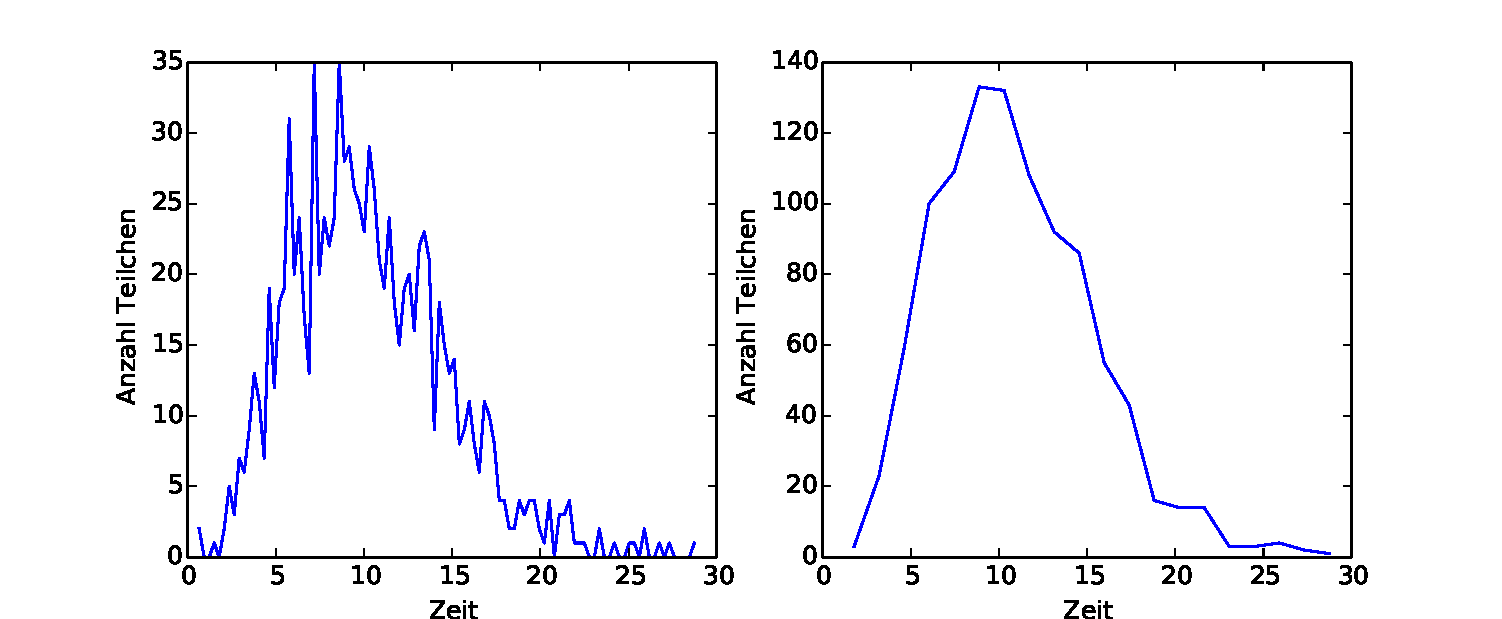
\includegraphics[width = \textwidth]{bilder/zeiten_zusammenfassen}\\
  \caption[Zeiten zusammenfassen]{Beispielpeak vor (links) und nach (rechts) der Zusammenfassung der Datenpunkte}
  \label{zeiten_zusammenfassen}
\end{figure}

Bei der Simulation, welche die Peaks in Abbildung \ref{zeiten_zusammenfassen} erzeugt hat, wurden $1000$ Teilchen simuliert. Es ist auf den ersten Blick nicht klar, wo sich die Maximalstelle des Peaks befindet, sowohl bei $t_1 = 7$ als auch bei $ t_2 = 8,5$ erreicht die Kurve ihren Maximalwert. Nach der Zusammenfassung von Ankunftszeiten wird klar, dass die Maximalstelle eher bei $t_2 = 8,5$ liegen muss. Die Berechnung der Lage der Peaks bezieht sich daher auf die zusammengefassten Daten.

Die Lage des Peaks und damit seine Retentionszeit bestimmt sich als am häufigsten vorkommende Ankunftszeit bei der Teilchensimulation bzw. als Lage des Maximalwertes beim PAA.

Für die Bestimmung von Interquartilsabstand und Quartilskoeffizient müssen zunächst die Quartile der Verteilung berechnet werden. Daraus lassen sich die beiden Werte direkt mit den in Kapitel \ref{chapter:gru} angegebenen Formeln berechnen. 
